% HOMIE final-year project report. Compile with XeLaTeX (Overleaf) or Tectonic.
% All text, author details, tables and TikZ figures are editable.
\documentclass[12pt,a4paper,oneside]{report}
\usepackage[margin=28mm,top=27mm,bottom=25mm,headheight=16pt]{geometry}
\usepackage[T1]{fontenc}
\usepackage{mathptmx}
\usepackage{graphicx,xcolor,booktabs,tabularx,array,amsmath}
\usepackage{setspace,fancyhdr,titlesec,enumitem,tikz,caption}
\usetikzlibrary{arrows.meta,positioning}
\usepackage[hidelinks,hypertexnames=false]{hyperref}
\definecolor{institution}{RGB}{24,61,119}
\definecolor{rulecolour}{RGB}{112,70,31}
\newcommand{\ProjectTitle}{HOMIE: Machine Learning-Based Transaction Risk Assessment on Solana}
\newcommand{\AcademicYear}{2026--27}
\newcommand{\GuideName}{Mr. Manjunath Prasad}
\newcommand{\AuthorTable}{\begin{tabular}{ll}\textbf{Bharath Kumar Shetty}&4MT23AI013\\\textbf{Deepthi P. Salian}&4MT23AI017\\\textbf{Shreya Shetty}&4MT23AI051\\\textbf{Swaroop Nellitheertha}&4MT23AI056\end{tabular}}
\setstretch{1.15}
\setlength{\parindent}{0pt}
\setlength{\parskip}{4pt}
\setlength{\emergencystretch}{2em}
\setlist{nosep,leftmargin=*}
\pagestyle{fancy}\fancyhf{}
\fancyhead[L]{\scriptsize\bfseries\itshape HOMIE: TRANSACTION RISK ASSESSMENT ON SOLANA}
\fancyfoot[L]{\scriptsize Dept. of AI\&ML, MITE, Moodbidri}
\fancyfoot[R]{\scriptsize Page -- \thepage}
\renewcommand{\headrulewidth}{0.5pt}\renewcommand{\footrulewidth}{0.5pt}
\fancypagestyle{plain}{\fancyhf{}\fancyhead[L]{\scriptsize\bfseries\itshape HOMIE: TRANSACTION RISK ASSESSMENT ON SOLANA}\fancyfoot[L]{\scriptsize Dept. of AI\&ML, MITE, Moodbidri}\fancyfoot[R]{\scriptsize Page -- \thepage}}
\titleformat{\chapter}[display]{\bfseries\large}{CHAPTER \thechapter}{12pt}{\centering\LARGE}
\titlespacing*{\chapter}{0pt}{8pt}{16pt}
\titlespacing*{\section}{0pt}{10pt}{4pt}
\titleformat{\section}{\large\bfseries}{\thesection}{0.7em}{}
\captionsetup{font=small,labelfont=bf}
\newcolumntype{Y}{>{\raggedright\arraybackslash}X}
\newcommand{\PageBorder}{\begin{tikzpicture}[remember picture,overlay]\draw[line width=1pt] ([xshift=13mm,yshift=-13mm]current page.north west) rectangle ([xshift=-13mm,yshift=13mm]current page.south east);\draw[gray,line width=.4pt] ([xshift=15mm,yshift=-15mm]current page.north west) rectangle ([xshift=-15mm,yshift=15mm]current page.south east);\end{tikzpicture}}
\begin{document}
\begin{titlepage}\PageBorder\centering\setstretch{1.0}\setlength{\parskip}{0pt}\fontsize{11}{13}\selectfont
{\color{institution}\large\bfseries VISVESVARAYA TECHNOLOGICAL UNIVERSITY\par}
Jnana Sangama, Belagavi -- 590018\par\vspace{5mm}
\includegraphics[height=25mm]{assets/vtu.png}\par\vspace{4mm}
{\large\bfseries A Project Report\par}on\par\vspace{3mm}
{\Large\bfseries ``\ProjectTitle''\par}\vspace{5mm}
Submitted in partial fulfilment of the requirements for the award of\par
\textbf{Bachelor of Engineering}\par in\par
\textbf{ARTIFICIAL INTELLIGENCE AND MACHINE LEARNING}\par\vspace{5mm}
Submitted by\par\vspace{2mm}\AuthorTable\par\vspace{6mm}
Under the guidance of\par{\large\bfseries\GuideName\par}\vspace{5mm}
\includegraphics[height=22mm]{assets/mite.png}\par\vspace{3mm}
{\color{institution}\bfseries DEPARTMENT OF ARTIFICIAL INTELLIGENCE\par AND MACHINE LEARNING\par}\vspace{3mm}
{\color{institution}\large\bfseries MANGALORE INSTITUTE OF\par TECHNOLOGY \& ENGINEERING\par}
Moodbidri, Karnataka\par\vfill{\large\AcademicYear\par}
\end{titlepage}
\pagenumbering{roman}
\begingroup\setstretch{1.05}\setlength{\parskip}{4pt}
\thispagestyle{empty}\PageBorder
\begin{center}{\color{institution}\large\bfseries MANGALORE INSTITUTE OF\par TECHNOLOGY \& ENGINEERING}\par
Department of Artificial Intelligence and Machine Learning\par\vspace{5mm}
\includegraphics[height=23mm]{assets/mite.png}\par\vspace{6mm}{\LARGE\bfseries CERTIFICATE}\end{center}\vspace{6mm}
This is to certify that the project entitled \textbf{``\ProjectTitle''} is the project work carried out by the following students in partial fulfilment of the requirements for the award of the Bachelor of Engineering degree in Artificial Intelligence and Machine Learning of Visvesvaraya Technological University, Belagavi, during the academic year \AcademicYear.
\begin{center}\AuthorTable\end{center}
The report is submitted for examination under the guidance of \textbf{\GuideName}.
% Certificate is an unsigned submission form. Obtain actual institutional signatures.
\vspace{12mm}
\begin{tabularx}{\textwidth}{YYY}
\hrulefill&\hrulefill&\hrulefill\\
\GuideName&Head of Department&Principal\\
Project Guide&&
\end{tabularx}
\vspace{10mm}\textbf{External examiners}\par
\begin{tabularx}{\textwidth}{Y Y}Name&Signature\\[9mm]1.\ \hrulefill&\hrulefill\\[9mm]2.\ \hrulefill&\hrulefill\end{tabularx}
\clearpage\endgroup
\chapter*{ABSTRACT}\addcontentsline{toc}{chapter}{Abstract}
HOMIE is a machine learning-based system for studying transaction execution risk on Solana. The project addresses transactions whose first signer has no available outcome history in the sampled data. It examines whether earlier outcomes involving other accounts that a transaction may modify provide useful predictive information.

The system constructs chronological account-participation features from public SolArchive records and trains histogram gradient boosting classifiers. A baseline uses transaction structure, signer history and read-only account context. The proposed feature extension adds non-signer writable-account history. A one-hour outcome delay prevents the current transaction or immature outcomes from entering its features. A stronger comparison supplies the same learned account-identity score to both models.

On the reserved first-appearance evaluation of 17,904 transactions, average precision increases from 0.1688 to 0.2004. A further test on 19,515 first appearances increases average precision from 0.2207 to 0.2393. The project also implements a web application with historical replay, actual model inference, live transfer checks, experimental live scores and decision-to-receipt recording. A controlled local-validator experiment verifies that a landed execution failure can incur a fee, while normal preflight can reject the same error without a fee.

The principal result is improved historical failure ranking under missing signer history. The implementation makes this result inspectable through a working application, while distinguishing model scores, network checks and observed transaction outcomes.

\textbf{Keywords:} Solana, machine learning, transaction failure, histogram gradient boosting, account history, temporal evaluation.
\chapter*{ACKNOWLEDGEMENT}\addcontentsline{toc}{chapter}{Acknowledgement}
We express our gratitude to our project guide, \GuideName, for guidance during the project. We thank the Department of Artificial Intelligence and Machine Learning at Mangalore Institute of Technology \& Engineering for providing the academic environment for this work.

We acknowledge the maintainers of SolArchive for making blockchain records publicly accessible, and the developers of Solana, scikit-learn and the open-source tools used in the implementation. We also thank our families and classmates for their support.
\vspace{12mm}\begin{flushright}Bharath Kumar Shetty\\Deepthi P. Salian\\Shreya Shetty\\Swaroop Nellitheertha\end{flushright}
\tableofcontents\listoffigures\listoftables
\clearpage\pagenumbering{arabic}
\chapter{INTRODUCTION}
\section{Project overview}
HOMIE uses earlier Solana records to rank transactions by execution-failure risk. Transactions may transfer SOL or interact with blockchain programs.

A wallet may have no usable history in the collected sample. However, the accounts involved in its transaction may have appeared in other transactions. HOMIE uses these shared histories as additional input to a machine learning model. Here, an account is a blockchain data address; it does not necessarily represent another person's wallet.
\section{Problem statement}
Signer-history models have little direct evidence when a signer has no available outcomes. The research question is: \emph{Does non-signer writable-account history improve failure ranking beyond transaction structure, signer history, read-only context and a learned identity control?}
\section{Objectives}
\begin{enumerate}
\item Construct reproducible features from public transaction records using only earlier available outcomes.
\item Compare a baseline and a writable-context model on chronological test periods.
\item Evaluate first-appearance transactions separately from aggregate performance.
\item Implement a usable interface for inference, transfer checks and traceable outcome recording.
\item Verify the fee mechanism using an isolated local validator.
\end{enumerate}
\section{Scope and contribution}
HOMIE retains the name of the original DeFi-companion concept, but its implemented focus is transaction-risk assessment. The work contributes an empirical evaluation of account-context features and an integrated prototype. Histogram gradient boosting is an established algorithm; the research contribution is the feature comparison and evaluation setting, rather than a newly invented classifier.

The predicted label is execution failure, not fraud, malicious intent or investment risk. ``Cold history'' means unavailable signer outcomes in the sampled replay; it does not establish that a wallet is newly created on Solana.
\chapter{LITERATURE SURVEY}
\section{Related work and technical foundations}
Zheng et al. study failed Solana transactions through large-scale measurements of initiators, programs and error patterns~\cite{zheng}. Their work establishes transaction failures as an empirical research subject. HOMIE focuses more narrowly on prediction when signer history is unavailable and on testing explicit shared-account history.

Solana's official documentation describes transaction fees and the RPC simulation interface~\cite{fees,simulation,send}. Simulation executes a candidate against a particular state; a statistical history model estimates patterns from past observations. These are different sources of information and require separate evaluation.

The scikit-learn histogram gradient boosting classifier provides the implemented tabular learning method~\cite{hgb}. Public SolArchive records supply the historical data~\cite{archive}.
\begin{table}[ht]\centering\caption{Relationship between existing resources and HOMIE}
\small\begin{tabularx}{\textwidth}{p{32mm}YY}\toprule
Resource&Relevant contribution&HOMIE focus\\\midrule
Solana failure study&Characterisation of failed transactions&Prediction under missing signer history\\
Solana RPC simulation&Execution check against current state&Displayed alongside independent ML scores\\
Histogram gradient boosting&Established tabular classifier&Controlled account-history feature comparison\\
SolArchive&Public transaction archive&Chronological sampled evaluation\\\bottomrule\end{tabularx}\end{table}
\section{Research position}
The tested hypothesis is that explicit writable-account participation summaries provide incremental ranking signal. A role-tagged identity learner is supplied to both compared models to make simple identity memorisation a stronger baseline. The positive results support this bounded empirical contribution; they do not establish universal novelty across all blockchain prediction research.
\chapter{SYSTEM REQUIREMENTS}
\section{Software used}
\begin{table}[ht]\centering\caption{Implemented technology stack}
\begin{tabularx}{\textwidth}{p{38mm}Y}\toprule Component&Technology and purpose\\\midrule
Data processing&Python, pandas, NumPy and PyArrow for archive extraction and features\\
Machine learning&scikit-learn histogram gradient boosting; SGD logistic identity control; isotonic calibration follow-up\\
Backend&FastAPI served with Uvicorn\\
Interface&Browser-based HTML, CSS and JavaScript\\
Study storage&SQLite for immutable decisions and separately attached receipts\\
Blockchain access&Solana JSON-RPC for blocks, balances, fee quotes and simulation\\
Verification&pytest and an isolated Solana local validator\\\bottomrule\end{tabularx}\end{table}
\section{Functional requirements}
The system must support historical replay, fitted-model inference, public-history refresh, native SOL transfer checks and outcome recording. It must report whether data is fresh enough for live scoring. It must preserve the exact candidate message and model provenance before associating a later receipt with a decision.
\section{Operating requirements}
Historical experiments require local storage for selected archive data and sufficient memory for feature tables. Live checks require an Internet connection and an available RPC endpoint. A browser and the Python environment run the application; local fee verification additionally requires a Solana validator installation. Minimum hardware throughput has not been benchmarked, so no unsupported minimum performance guarantee is specified.
\section{Reliability requirements}
Insufficient or stale live history must withhold an ML score. Missing network responses must remain incomplete checks. Unknown receipt outcomes must remain unknown. The web application performs checks without signing or broadcasting transactions.
\chapter{SYSTEM DESIGN}
\section{Architecture}
The architecture separates historical experimentation from live transfer analysis. Both routes reuse participation-history features, but live scores are experimental because current sampling and network conditions differ from the historical training data.
\begin{figure}[ht]\centering\includegraphics[width=\textwidth,height=.70\textheight,keepaspectratio]{assets/architecture.png}\caption{Implemented research and application architecture.}\end{figure}
\clearpage
\section{Transaction-check workflow}
\begin{figure}[ht]\centering
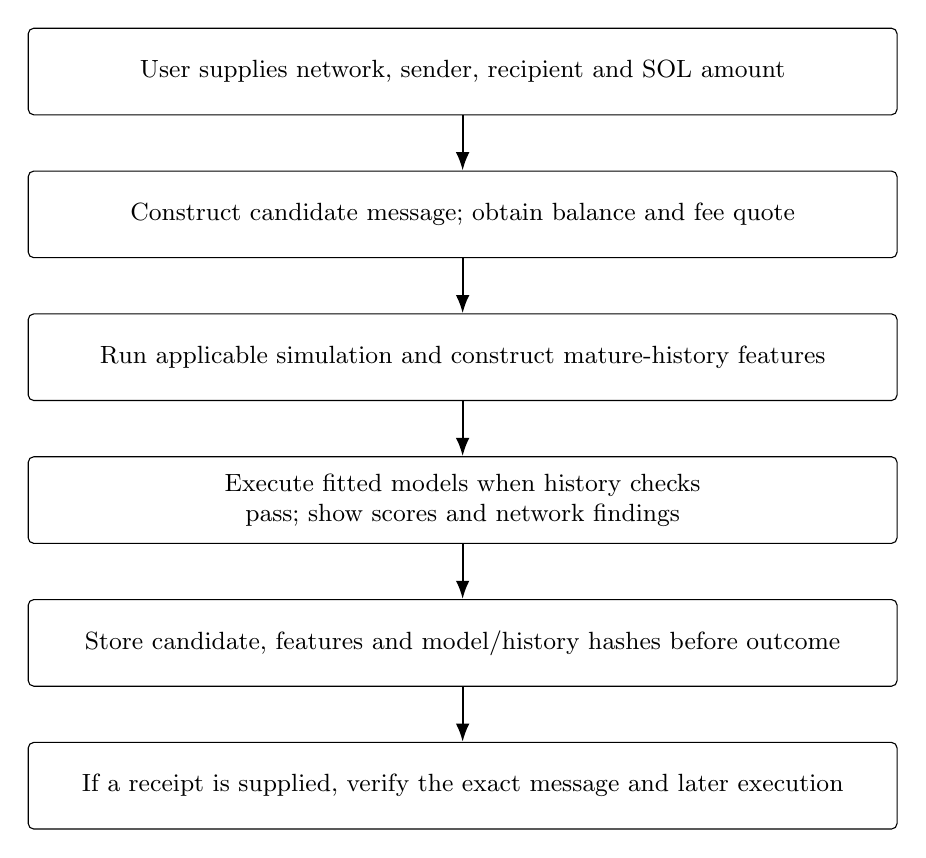
\begin{tikzpicture}[node distance=7mm,box/.style={draw,rounded corners=2pt,align=center,text width=108mm,minimum height=11mm,font=\small},arr/.style={-{Latex},thick}]
\node[box](a){User supplies network, sender, recipient and SOL amount};
\node[box,below=of a](b){Construct candidate message; obtain balance and fee quote};
\node[box,below=of b](c){Run applicable simulation and construct mature-history features};
\node[box,below=of c](d){Execute fitted models when history checks pass; show scores and network findings};
\node[box,below=of d](e){Store candidate, features and model/history hashes before outcome};
\node[box,below=of e](f){If a receipt is supplied, verify the exact message and later execution};
\foreach \x/\y in {a/b,b/c,c/d,d/e,e/f}\draw[arr](\x)--(\y);
\end{tikzpicture}\caption{Live checking and outcome-recording workflow.}\end{figure}
\section{Data and responsibility boundaries}
The archive provides transaction outcomes for retrospective evaluation. The RPC service supplies present network observations. The ML component consumes account-role and historical features; transfer amount is handled by the balance and simulation checks. The study store preserves the decision before the receipt is attached. This separation makes it possible to identify which component produced each finding.
\chapter{METHODOLOGY AND IMPLEMENTATION}
\section{Data collection and labels}
The historical source is SolArchive, licensed CC BY 4.0~\cite{archive}. The pinned dataset revision is:\par
{\small\texttt{6588cad2832e62be03972ac80d69c6af11d631c8}}\par
 One selected Parquet row group per date is used. The initial four windows contain 1,588,408 raw records before duplicate removal and exclusions. This is a sparse sample, not complete chain coverage.

Selected fields include transaction signature, account addresses and roles, block timestamp, block slot and execution status. The target is binary execution failure. Original instruction payloads, unlanded attempts and paid fee amounts are not available in the selected historical table.
\section{Chronological features}
At transaction time $t$, an earlier outcome contributes only if its inclusion timestamp is at least one hour earlier. Features are computed before the current outcome is scheduled for later availability. The first six training hours build history. Rows whose labels would cross the next date boundary are purged from training and validation.

For account $a$ in role $r$, the smoothed historical failure rate is
\begin{equation}q_r(a,t)=\frac{f_r(a,t)+20b(t)}{n_r(a,t)+20},\qquad b(t)=\frac{F(t)+1}{N(t)+2}.\end{equation}
Here $f_r$ and $n_r$ are available failures and observations for that role; $F$ and $N$ are their global counterparts. Features summarise seen fractions, log counts and failure-rate mean, maximum, minimum and standard deviation. Ten common infrastructure addresses are excluded from contextual histories and represented through structural indicators.
\section{Learning algorithm}
Histogram gradient boosting combines successive decision trees to reduce classification loss. Numeric feature values are grouped into bins for efficient split selection~\cite{hgb}. Both primary models use the same classifier settings so the comparison concerns the added features.
\begin{table}[ht]\centering\caption{Histogram gradient boosting configuration}
\begin{tabular}{ll}\toprule Parameter&Value\\\midrule Maximum iterations&150\\Maximum leaf nodes&15\\Minimum samples per leaf&40\\L2 regularisation&5\\Early stopping&Disabled\\Seeds averaged&42, 73, 101\\\bottomrule\end{tabular}\end{table}
The fits are effectively deterministic; the three seeds are not independent experimental replications. The baseline includes structure, signer history and read-only/template history. The context model adds non-signer writable-account history.
\section{Identity control and calibration}
A stronger comparison uses an SGD logistic learner with role-tagged identities and read-only templates hashed into $2^{20}$ dimensions. Binary features are L2 normalised; regularisation is 0.0001. Its chronological predictions are supplied to both gradient boosting models. Labels mature after one hour, with ten-minute learning batches introducing a small additional update delay.

A separate operational follow-up fits isotonic calibration on early cold-history validation data and chooses thresholds on later validation data. This follow-up is distinct from the identity-controlled primary comparison. Live application outputs remain experimental raw scores rather than validated live failure probabilities.
\section{Evaluation windows}
\begin{table}[ht]\centering\caption{Chronological experimental windows (2025)}
\begin{tabular}{llll}\toprule Window&Training&Validation&Testing\\\midrule Initial&Nov. 1&Nov. 2&Nov. 3\\Confirmation&Nov. 8&Nov. 9&Nov. 10\\Extension&Nov. 22&Nov. 23&Nov. 24\\Reserved refined&Nov. 29&Nov. 30&Dec. 1\\Further test&Dec. 3&Dec. 4&Dec. 5\\\bottomrule\end{tabular}\end{table}
Average precision (AP) measures how well failures rank ahead of successful transactions across score cut-offs. It is not classification accuracy. AUROC, Brier loss, recall and false-positive rate provide complementary information. Paired bootstrap resampling of hourly blocks uses 500 draws to estimate uncertainty in AP differences.
\section{Application implementation}
The FastAPI application provides historical replay at \texttt{/}, fitted inference at \texttt{/predict}, transfer checks at \texttt{/check}, integrated analysis at \texttt{/live} and fee verification at \texttt{/fee-proof}. The backend reconstructs plain SOL transfer messages, handles exact lamport amounts and queries Solana RPC.

Live snapshots must meet freshness and history requirements: at least 100 records spanning six hours, with a snapshot no older than one hour. Only outcomes aged at least one hour enter history. The same extractor used in research builds live features. Scores are withheld when checks fail.

SQLite records candidate-message, feature, model and history hashes. Database triggers protect decisions and receipts from mutation. Receipt verification checks the exact candidate message, signature, later slot and timestamp, and consistency of fee and balance changes. An unrelated receipt cannot be used as evidence for a decision.
\chapter{TESTING}
\section{Verification strategy}
Targeted automated tests cover feature timing, inference, transfer-message construction, policy arithmetic and receipt integrity. The recorded verification run reports 45 passing targeted tests. This count refers to the selected project checks, not a claim about every test in the repository.
\begin{table}[ht]\centering\caption{Implemented checks and recorded verification}
\small\begin{tabularx}{\textwidth}{p{35mm}YY}\toprule Area&Expected behaviour&Recorded verification\\\midrule
History maturity&Exclude current and immature outcomes&Targeted tests passed\\
Freshness and network&Withhold scores for stale or mismatched data&Targeted tests passed\\
Insufficient balance&Show amount-plus-fee shortfall&Live HTTP case verified\\
Rent constraint&Surface simulation error&Live HTTP case verified\\
Valid small transfer&Show simulation pass at checked state&Live HTTP case verified\\
Read-only operation&Do not broadcast from web checks&Targeted tests and HTTP checks\\
Receipt integrity&Reject unrelated, old or duplicate receipts&Targeted tests passed\\
Local receipt flow&Attach matching later receipt to stored decision&Local validator verification\\\bottomrule\end{tabularx}\end{table}
\section{Fee-mechanism experiment}
An isolated local validator and throwaway keys are used to compare a deliberately invalid transfer under different submission conditions. Normal preflight rejects the invalid candidate without a paid transaction fee. In a test-only path, disabling preflight allows a landed execution failure; the receipt and balance change record 5,000 lamports. A successful transfer separately checks principal-plus-fee accounting.

This experiment verifies fee behaviour and traceable outcomes. It does not establish that the ML model outperforms ordinary preflight. The local validator uses test funds and the production web flow does not bypass preflight or submit transactions.
\chapter{RESULTS AND DISCUSSION}
\section{Historical ranking results}
\begin{table}[ht]\centering\caption{Cold-history AP without the identity-score control}
\begin{tabular}{lrrr}\toprule Test date&Transactions&Baseline AP&Context AP\\\midrule Nov. 3&19,621&0.3193&0.3787\\Nov. 10&20,636&0.2249&0.2514\\Nov. 24&21,028&0.2052&0.2231\\Dec. 1&19,577&0.1734&0.2185\\\bottomrule\end{tabular}\end{table}
All four point estimates favour writable context, but the November 24 interval for the difference crosses zero. Results therefore do not imply an advantage in every period.
\begin{table}[ht]\centering\caption{First-appearance results with the identity-score control}
\small\begin{tabularx}{\textwidth}{lrrrY}\toprule Test&Rows&Baseline AP&Context AP&AP gain, 95\% interval\\\midrule Dec. 1&17,904&0.1688&0.2004&0.0316 [0.0168, 0.0501]\\Dec. 5&19,515&0.2207&0.2393&0.0186 [0.0095, 0.0288]\\\bottomrule\end{tabularx}\end{table}
The reserved December 1 endpoint has 5.88\% failure prevalence. Its AUROC rises from 0.7288 to 0.7545. The further December 5 result also supports additional ranking signal beyond the shared identity control.
\section{Ranking versus warning decisions}
On December 1, inherited validation thresholds yield false-positive rates of 22.66\% for the baseline and 28.65\% for the context model. Recall rises from 50.90\% to 64.48\%, but this comparison does not hold false positives constant. Brier loss worsens from 0.0967 to 0.1218. Better ranking therefore does not automatically mean better calibrated probabilities or a better warning policy.

In the interface, a displayed score such as 30.8\% is a model output for one transaction, not 30.8\% model accuracy. Whether a case is flagged depends on a threshold; judging a policy requires outcomes across many transactions and attention to both missed failures and false alarms.
\section{Fee-policy and local results}
\begin{table}[ht]\centering\caption{Measured local fee-mechanism outcomes}
\begin{tabularx}{\textwidth}{Y r}\toprule Local condition&Paid fee (lamports)\\\midrule Check candidate and stop&0\\Normal preflight rejects invalid candidate&0\\Force landed execution failure in isolated test&5,000\\\bottomrule\end{tabularx}\end{table}
A retrospective policy audit covers 102,443 cold-history transactions with 6,410 failures. At an assumed false-warning cost five times a failed-attempt fee, context warnings cover 107 failures and 60 successes while missing 6,303 failures. Hypothetical utility is $107-5(60)=-193$ fee units. These units are assumed costs, not measured SOL savings.
\section{Practical interpretation and limitations}
The implemented system provides an inspectable ML comparison, current balance and simulation checks, and a record linking decisions to verified receipts. This is useful for studying failure risk and diagnosing supported transfer problems before submission.

The historical sample is sparse and originates from one provider. Inclusion timestamps approximate information availability rather than submission time. The selected table excludes unlanded attempts and full instruction payloads. Historical identity controls and participation features have slightly different update schedules. Live RPC sampling differs from training, and a simulation pass is state-dependent. Measured ML-driven fee savings and retry-time reductions are not established by the current experiments.
\chapter{CONCLUSION AND FUTURE SCOPE}
\section{Conclusion}
HOMIE implements an end-to-end transaction-risk research system on Solana. Public records are transformed into time-respecting account features, established machine learning models are compared, and predictions are exposed through an application with live checks and traceable outcomes.

The strongest finding is that writable-account participation history adds failure-ranking signal for sampled first-appearance signers, including comparisons with a learned identity control. The project also verifies the fee mechanism and the decision-to-receipt workflow. Its results distinguish predictive ranking from probability calibration and economic benefit.
\section{Future scope}
Further work can evaluate independent data sources and periods, align identity-learning update schedules, and test cold-specific calibration under changing conditions. A prospective study should compare candidates that pass normal preflight before measuring any incremental ML benefit. Broader transaction types, authorised wallet integration and measured user task times are additional extensions. These are extensions to the completed research prototype rather than results claimed in this report.
\renewcommand{\bibname}{REFERENCES}
\begin{thebibliography}{9}\addcontentsline{toc}{chapter}{References}
\bibitem{zheng} X. Zheng, Z. Wan, D. Lo, D. Xie and X. Yang, ``Why Does My Transaction Fail? A First Look at Failed Transactions on the Solana Blockchain,'' 2025. \url{https://arxiv.org/abs/2504.18055}. DOI: 10.1145/3728943.
\bibitem{archive} SolArchive, ``SolArchive transaction dataset,'' Hugging Face, CC BY 4.0. \url{https://huggingface.co/datasets/solarchive/solarchive}. Revision specified in Chapter 5.
\bibitem{hgb} scikit-learn developers, ``HistGradientBoostingClassifier,'' official API documentation. \url{https://scikit-learn.org/stable/modules/generated/sklearn.ensemble.HistGradientBoostingClassifier.html}.
\bibitem{fees} Solana Foundation, ``Fees,'' official documentation. \url{https://solana.com/docs/core/fees}.
\bibitem{simulation} Solana Foundation, ``simulateTransaction,'' RPC documentation. \url{https://solana.com/docs/rpc/http/simulatetransaction}.
\bibitem{send} Solana Foundation, ``sendTransaction,'' RPC documentation. \url{https://solana.com/docs/rpc/http/sendtransaction}.
\end{thebibliography}
\end{document}
